\documentclass[10pt]{beamer}
\usepackage{ceai-beamer}
\usepackage{ragged2e}
\usepackage{subcaption}
\usepackage{tikz}
\usetikzlibrary{positioning,arrows.meta,shapes.multipart}

% Footnote/source text styling
\definecolor{footnotepurple}{RGB}{128,0,128}
\newcommand{\sourcesnote}[1]{{\footnotesize\color{footnotepurple}#1}}

\title{CE 488/5588: Applied AI for Engineering\\ \large Topic 3: ML Paradigms and Formalisms}
\author{}
\institute{}
\date{}

\begin{document}

\begin{frame}
    \titlepage
\end{frame}

\begin{frame}{Outline}
    \justifying
    \tableofcontents
\end{frame}

\begin{frame}{Learning Objectives}
    \justifying
    \begin{itemize}
        \item Map the three fundamental machine learning paradigms and their data assumptions.
        \item Distinguish discriminative and generative learning formalisms with concrete examples.
        \item Explain how decision boundaries, loss functions, and Bayes' rule guide model design.
        \begin{itemize}
            \item These objectives frame the rest of the course sequence and model choices.
        \end{itemize}
    \end{itemize}
\end{frame}

\section{Machine Learning: A Big-Picture View}

\begin{frame}{Machine Learning as Data-Enabled AI}
    \justifying
    \begin{itemize}
        \item Machine learning (ML) is the most robust and widely adopted arena of modern AI.
        \item Deep learning and generative AI are recent advances within this data-enabled paradigm.
        \begin{itemize}
            \item The dominance of ML reflects the practical success of learning from data at scale.
        \end{itemize}
    \end{itemize}
\end{frame}

\begin{frame}{Inductive vs. Deductive Reasoning in ML}
    \justifying
    \begin{itemize}
        \item ML is primarily \textbf{inductive} during training: it learns patterns from data.
        \item ML is primarily \textbf{deductive} during inference: it applies learned rules to new inputs.
        \begin{itemize}
            \item This dual structure aligns with how humans generalize and then apply knowledge - \textit{with the least complexity}.
        \end{itemize}
    \end{itemize}
\end{frame}

\begin{frame}{Two Fundamental Questions}
    \justifying
    \begin{itemize}
        \item How many machine learning paradigms exist?
        \item How do we formulate learning, i.e., what are the basic learning formalisms?
        \begin{itemize}
            \item These questions define the conceptual map for the rest of the course.
        \end{itemize}
    \end{itemize}
\end{frame}

\begin{frame}{Three Fundamental ML Paradigms}
    \justifying
    Canonical definitions used across ML curricula.
    \begin{itemize}
        \item Supervised Learning: learn from labeled examples.
        \item Unsupervised Learning: discover structure in unlabeled data.
        \item Reinforcement Learning: learn by interacting with an environment.
        \begin{itemize}
            \item Yet, is it still data-driven ML?
        \end{itemize}
\end{itemize}
    \vspace{0.5em}
    {\footnotesize Sources: \url{https://www.cs.cornell.edu/courses/cs4780/2018fa/lectures/lecturenote01_MLsetup.html};
    \url{https://introml.mit.edu/_static/spring24/LectureNotes/chapter_Unsupervised_Learning.pdf};
    \url{https://introml.mit.edu/notes/reinforcement_learning.html}}
\end{frame}

\begin{frame}{Data-Driven vs. Interaction-Driven Learning}
    \justifying
    \begin{itemize}
        \item Supervised and unsupervised learning are data-driven paradigms.
        \item Reinforcement learning is interaction-driven and generates data through trial and error.
        \begin{itemize}
            \item Interaction changes the distribution of data the agent experiences.
            \item So, RL remains data-enabled. 
        \end{itemize}
        \item Other types include semi-supervised, weakly supervised, and self-supervised learning (\textit{which is NOT unsupervised learning}).
    \end{itemize}
\end{frame}

\begin{frame}{Two Learning Formalisms}
    \justifying
    \begin{itemize}
        \item Discriminative learning: learn decision boundaries or $P(c \mid x)$ directly.
        \item Generative learning: model how data are generated via $p(x \mid c)$ and $P(c)$.
        \begin{itemize}
            \item The formalism determines what the model learns from the same data.
        \end{itemize}
    \end{itemize}
\end{frame}



\begin{frame}{Paradigms and Formalisms (Map)}
\centering
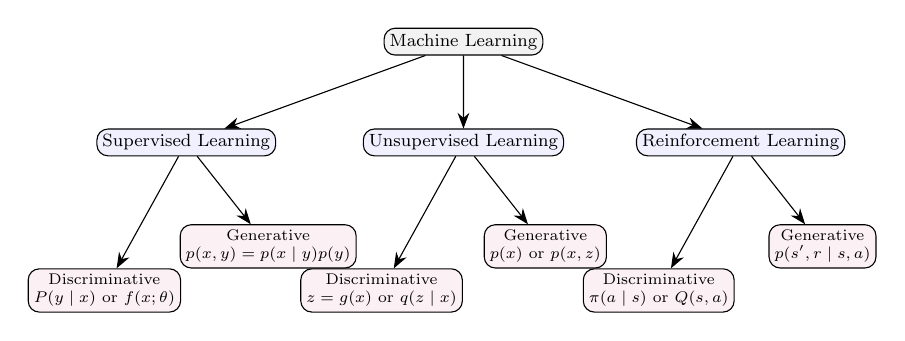
\begin{tikzpicture}[
    grow=down,
    scale=0.8,
    transform shape,
    edge from parent/.style={draw,-{Stealth[length=2.0mm]}},
    box/.style={draw,rounded corners,align=center,inner sep=2.5pt},
    root/.style={box,fill=gray!10,font=\footnotesize},
    par/.style={box,fill=blue!6,font=\footnotesize},
    leaf/.style={box,fill=purple!6,font=\scriptsize},
    level 1/.style={level distance=1.6cm, sibling distance=4.4cm},
    level 2/.style={level distance=2.0cm, sibling distance=2.6cm}
]

\node[root]{Machine Learning}
    child {node[par]{Supervised Learning}
        child {node[leaf,yshift=-0.35cm]{Discriminative\\
            $P(y\mid x)$ or $f(x;\theta)$}}
        child {node[leaf,yshift=0.35cm]{Generative\\
            $p(x,y)=p(x\mid y)p(y)$}}
    }
    child {node[par]{Unsupervised Learning}
        child {node[leaf,yshift=-0.35cm]{Discriminative\\
            $z=g(x)$ or $q(z\mid x)$}}
        child {node[leaf,yshift=0.35cm]{Generative\\
            $p(x)$ or $p(x,z)$}}
    }
    child {node[par]{Reinforcement Learning}
        child {node[leaf,yshift=-0.35cm]{Discriminative\\
            $\pi(a\mid s)$ or $Q(s,a)$}}
        child {node[leaf,yshift=0.35cm]{Generative\\
            $p(s',r\mid s,a)$}}
    };

\end{tikzpicture}
\end{frame}

\begin{frame}{Course Roadmap}
    \justifying
    \begin{itemize}
        \item Begin with supervised learning theories and models.
        \item Introduce unsupervised learning after supervised foundations.
        \item Discuss reinforcement learning briefly as a unique paradigm.
        \begin{itemize}
            \item Each paradigm will be explored with both discriminative and generative formalisms.
        \end{itemize}
    \end{itemize}
\end{frame}
\section{Thought Experiment}

\begin{frame}{Running Example: Drinking-Water Compliance}
    \justifying
    \begin{itemize}
        \item Supervised learning: each sample has an observed outcome (compliant vs. noncompliant), (safe vs. unsafe), or less techncial, (good vs. bad)
        \item Discriminative learning: map measurements directly to the label.
        \item Generative learning: model measurement distributions within each class.
        \begin{itemize}
            \item This example highlights how modeling choices shape inference.
        \end{itemize}
    \end{itemize}
\end{frame}

\begin{frame}{Drinking Water pH Compliance (Toy Example)}
    \justifying
    \begin{examplebox}{Toy Example}
        An engineer monitors drinking-water safety using pH values.
        The dataset includes measurements such as
        $\bm{x} = \{7.8, 5.9, 9.0, 6.0, 7.8, \cdots\}$ with $N = 100$ samples.
        The task is to decide whether a sample is compliant/safe or noncompliant/unsafe.
    \end{examplebox}
\end{frame}

\begin{frame}{Why This Thought Experiment?}
    \justifying
    \begin{itemize}
        \item The goal is not to predict yet, but to understand first - how can we predict?
        \item Each formalism learns different information from the same observations.
        \begin{itemize}
            \item This understanding informs model selection and interpretation in practice.
            \item In the next, we sidetrack a bit - starting thinking first how we can predict with the classical way (non-ML).
        \end{itemize}
    \end{itemize}
\end{frame}

\section{Rule-Based Decision Making and AI}

\begin{frame}{Classical Decision Making Without Learning}
    \justifying
    \begin{itemize}
        \item Symbolic AI (rule-based AI, GOFAI) encodes knowledge as explicit rules.
        \item Inference is primarily deductive, driven by human-designed logic.
        \begin{itemize}
            \item This was the dominant paradigm in early expert systems.
        \end{itemize}
    \end{itemize}
\end{frame}

\begin{frame}{Rule-Based Decision Function}
    \justifying
    \begin{examplebox}{Threshold Rule for pH}
        Acceptable drinking-water pH is often listed as approximately $6.5$ to $8.5$.
        We simplify this to a single threshold at the upper bound:
        \[
          F(pH) = \left\{
            \begin{array}{ll}
              \mathrm{C0: compliant/safe} & \text{if } pH < 8.5, \\
              \mathrm{C1: noncompliant/unsafe} & \text{if } pH \geq 8.5.
            \end{array}
          \right.
        \]
    \end{examplebox}
    \vspace{0.5em}
    \sourcesnote{Source: \url{https://www.epa.gov/sdwa/secondary-drinking-water-standards-guidance-nuisance-chemicals}}
\end{frame}

\begin{frame}{Decision Boundary Interpretation}
    \justifying
    \begin{itemize}
        \item The value $pH = 8.5$ acts as a decision boundary.
        \item A sample such as $\bm{x}[3] = 9.0$ is labeled noncompliant/unsafe.
        \begin{itemize}
            \item This is simple, transparent, and easy to apply at scale.
        \end{itemize}
    \end{itemize}
\end{frame}

\begin{frame}{Limitations of Rule-Based Decisions}
    \justifying
    \begin{itemize}
        \item Valid under ideal assumptions, but often inaccurate in practice.
        \item Real outcomes depend on measurement uncertainty and operational definitions.
        \begin{itemize}
            \item This motivates a data-driven machine learning approach.
        \end{itemize}
    \end{itemize}
\end{frame}

\section{Supervised Learning: Classification}

\begin{frame}{From Rules to Labeled Data}
    \justifying
    \begin{itemize}
        \item An inspector provides labels based on operational compliance.
        \item Labeled outcomes: $\bm{c} = \{1, 1, 1, 0, 1, \cdots\}$.
        \item $1$ denotes compliant/safe and $0$ denotes noncompliant/unsafe.
        \begin{itemize}
            \item Letting the data speak replaces rigid rules with learned boundaries.
        \end{itemize}
    \end{itemize}
\end{frame}

\begin{frame}{Observed pH Values and Labels}
    \justifying
    \begin{figure}
        \centering
        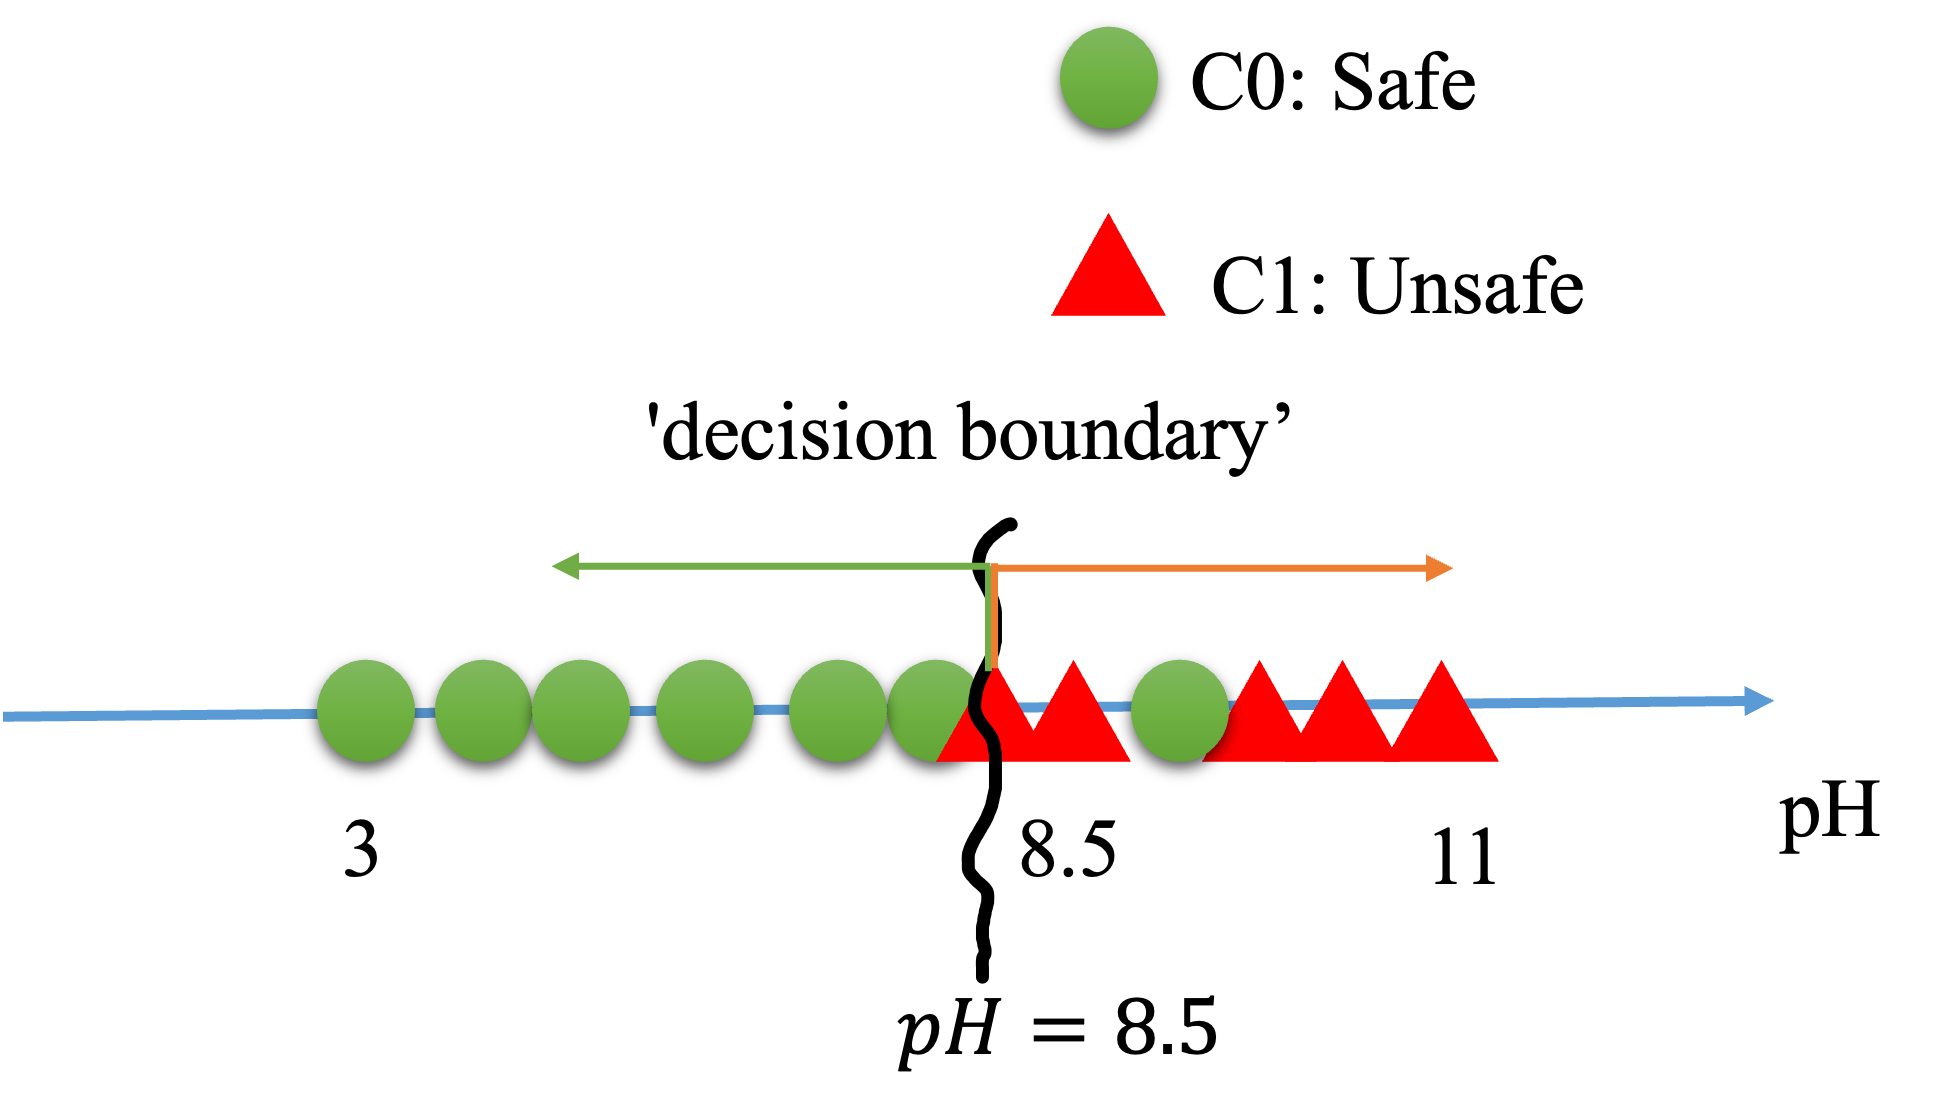
\includegraphics[width=0.7\textwidth]{../figs/pHvalues_2.png}
        \caption{Drinking-water pH measurements with a guessed decision boundary.}
    \end{figure}
\end{frame}

\begin{frame}{Why the Boundary Moves}
    \justifying
    \begin{itemize}
        \item A fixed threshold may not match observed outcomes.
        \item The effective boundary can shift with uncertainty and covariates.
        \begin{itemize}
            \item ML aims to resolve these disagreements using data-driven optimization.
        \end{itemize}
    \end{itemize}
\end{frame}

\begin{frame}{Labeled Dataset Definition}
    \justifying
    \begin{conceptbox}{Dataset}
        \[
        \bm{D} = \{ (x_i, c_i) \mid x_i \in [0, 10],\, c_i \in \{0, 1\},\, i = 1,2,\cdots,N \}
        \]
        Here, $x_i$ is a measurement (feature) and $c_i$ is its label.
    \end{conceptbox}
\end{frame}

\begin{frame}{Generic Binary Classifier}
    \justifying
    \begin{equation}
    m(x \mid \bm{w}) = \left\{
        \begin{array}{ll}
          c_1 & \text{if } f(x \mid \bm{w}) \geq \sigma, \\
          c_0 & \text{if } f(x \mid \bm{w}) < \sigma.
        \end{array}
    \right.
    \end{equation}
    \begin{itemize}
        \item $\bm{w}$ is the parameter vector of the decision function $f(x \mid \bm{w})$.
        \item $f(x \mid \bm{w}) - \sigma = 0$ defines the decision boundary.
    \end{itemize}
\end{frame}

\begin{frame}{From Thresholds to Learned Parameters}
    \justifying
    \begin{itemize}
        \item Rule-based approach: $f(x \mid \bm{w}) = \sigma$, actually without using $\bm{w}$ and $\sigma = 8.5$.
        \item General ML approach: $f(x \mid \bm{w}) = \sigma $, with a model parameter set $\bm{w}$ and $\sigma$ to be determined, and  $f(x \mid \bm{w}) -\sigma = 0$ can be a nonlinear boundary function.
        \begin{itemize}
            \item The threshold can be absorbed into $\bm{w}$ by augmenting features.
            \item $f(x \mid \bm{w}) = 0$ is then used($\sigma$ is part of $\bm{w}$)
        \end{itemize}
    \end{itemize}
\end{frame}

\begin{frame}{Classification in a Transformed Space}
    \justifying
    \begin{figure}
        \centering
        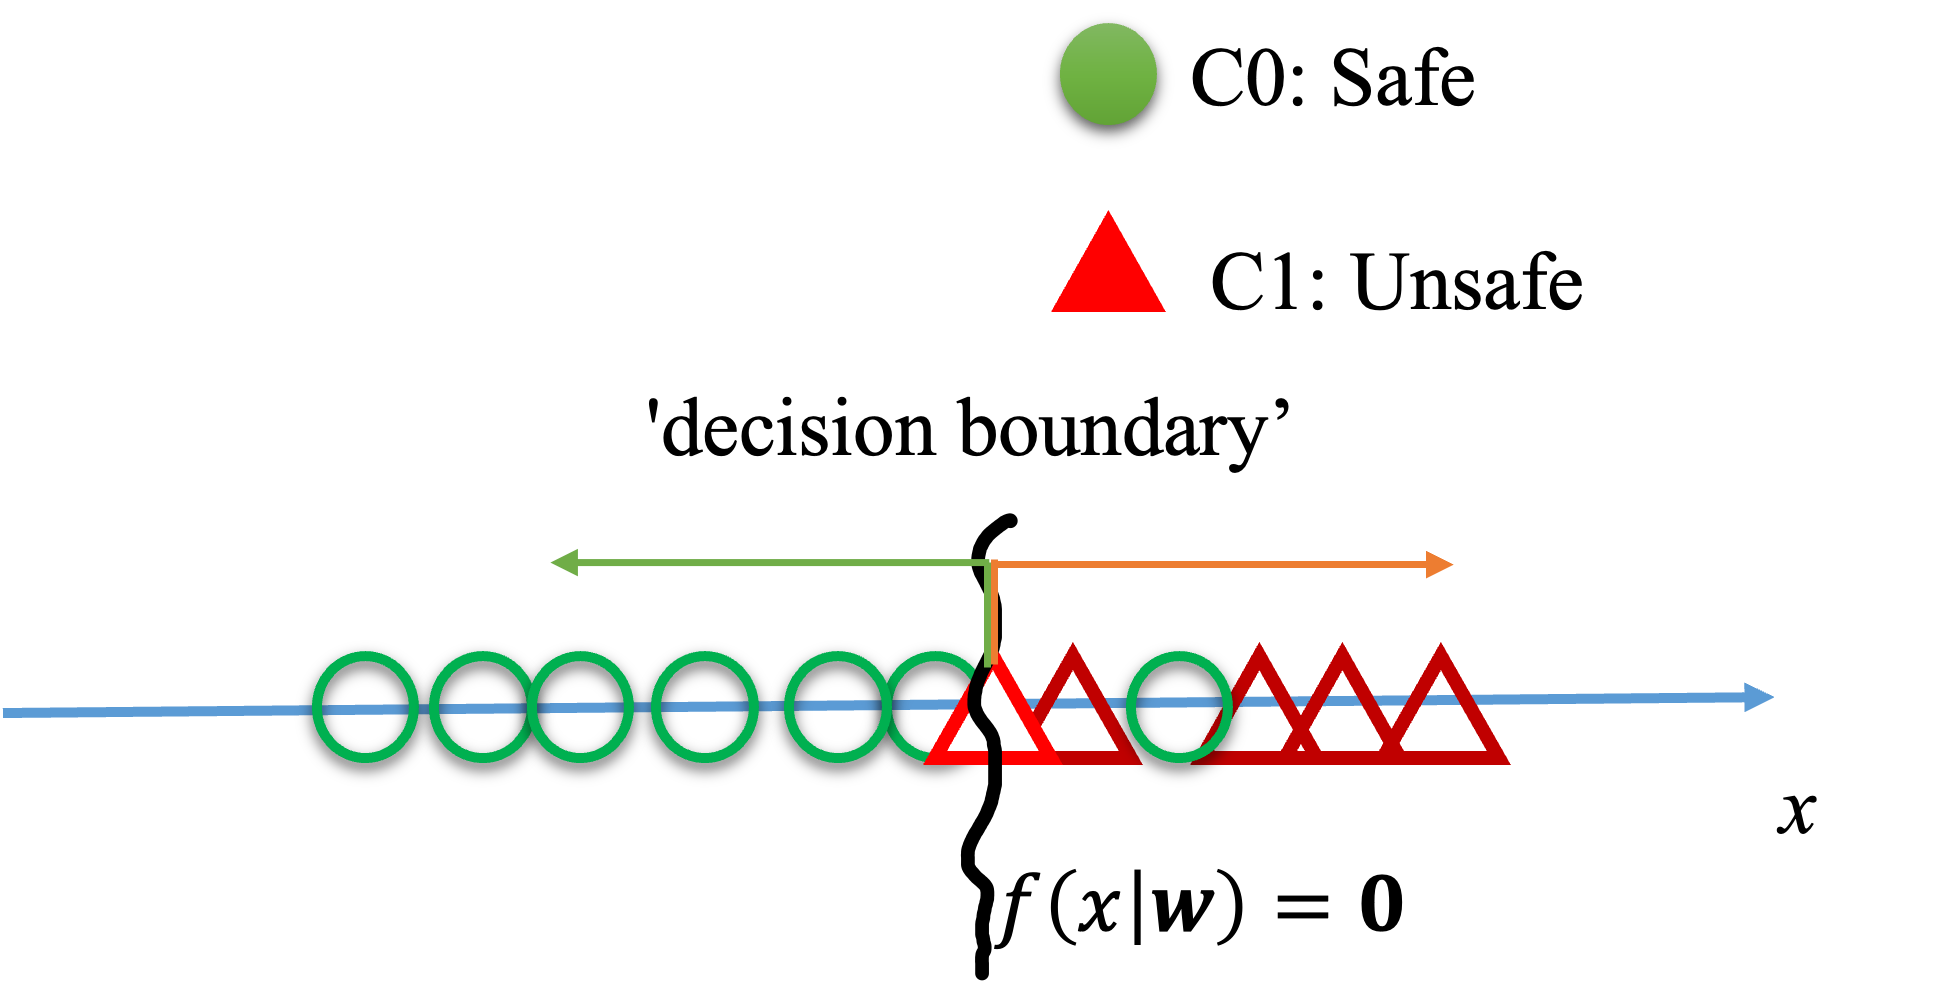
\includegraphics[width=0.7\textwidth]{../figs/pHvalues_transformed_2.png}
        \caption{Classification in a transformed space of $f(x \mid \bm{w})$.}
    \end{figure}
\end{frame}

\begin{frame}{Multi-Class Inference}
    \justifying
    Now, treating $f(x \mid \bm{w}) = 0$, as the boundary function, defining the decision boundary, we expect: 
    \begin{itemize}
        \item If $f(x \mid \bm{w}) > 0$ and if it is higher in the positive side, it is more convining (higher plausibility) that $x$ belongs to C1: unsafe
        \item If $f(x \mid \bm{w}) < 0$ and if it is lower in the negative side, it is more convining (higher plausibility) that $x$ belongs to C0: safe.
    \end{itemize}
    Combining them, we have
    \begin{equation}
        c^* = \mathrm{argmax}_c\, f(x \mid \bm{w})
    \end{equation}
    
     \begin{itemize}
        \item The predicted class is the one with the highest decision function value.
        \item The numeric value of $f(x \mid \bm{w})$ is often called a \textcolor{red}{\textit{score}}.
    \end{itemize}
\end{frame}

\section{Discriminative Learning}

\begin{frame}{Discriminative Learning Formulation}
    \justifying
    \begin{conceptbox}{Definition}
        Discriminative learning directly constructs a decision function and learns its parameters
        from labeled data via optimization.
    \end{conceptbox}
    \begin{itemize}
        \item The model focuses on mapping inputs to outputs, not on modeling data generation.
        \item Effectively, $f(x \mid \bm{w})$ is learned directly by deciding a model structure for $f(\cdot)$ and estimate the parameter set $\bm{w}$, WITHOUT learning how $x$ is generated. 
    \end{itemize}
\end{frame}

\begin{frame}{Learning - How? Generally, }
    \justifying
    We need to define Loss Functions and create an Optimization scheme.
    \begin{itemize}
        \item A loss function penalizes wrong predictions.
\begin{itemize}
    \item The simplest loss at an observation $(x_i, c_i)$ given a prediction $(x_i, c_i^p)$:
    \[
        l_i = | c_i - c_i^p|
        \]
        \item or 
          \[
        l_i = | c_i - c_i^p|^2
        \]

        (\textcolor{red}{squared loss is better or not?!})
   
\end{itemize}

        \item The total loss over the dataset is minimized to estimate $\bm{w}$.
        \begin{itemize}
            \item The choice of loss shapes the decision boundary and generalization behavior.
            \item  With the use of $c_i$ - the ground-truth label, it serves as a `teacher' or a supervision -- this is why we call it supervised learning!
        \end{itemize}
    \end{itemize}
\end{frame}

\begin{frame}{Classic Discriminative Models}
    \justifying
    \begin{itemize}
        \item Logistic regression (parametric).
        \item Feed-forward neural networks (parametric).
        \item Support vector machines (non-parametric).
        \begin{itemize}
            \item These models vary in flexibility and computational cost.
        \end{itemize}
    \end{itemize}

    \begin{itemize}
        \item At this moment, just undertand that a parametric model has a fixed-number of weights
        \item A non-parametric model has the number of model parametrers depending on the data size of $\mathcal{D}$.
    \end{itemize}
\end{frame}

\begin{frame}{From Scalar to Vector Features}
    \justifying
    \begin{itemize}
        \item Replace scalar $x$ with a feature vector $\bm{x} = [x; y]$.
        \item Example: pH ($x$) and PFAS level ($y$, part per millions) as two measurements.
        \begin{itemize}
            \item The decision boundary becomes a curve in 2-D space.
        \end{itemize}
    \end{itemize}
\end{frame}

\begin{frame}{Nonlinear Decision Boundary}
    \justifying
    \begin{figure}
        \centering
        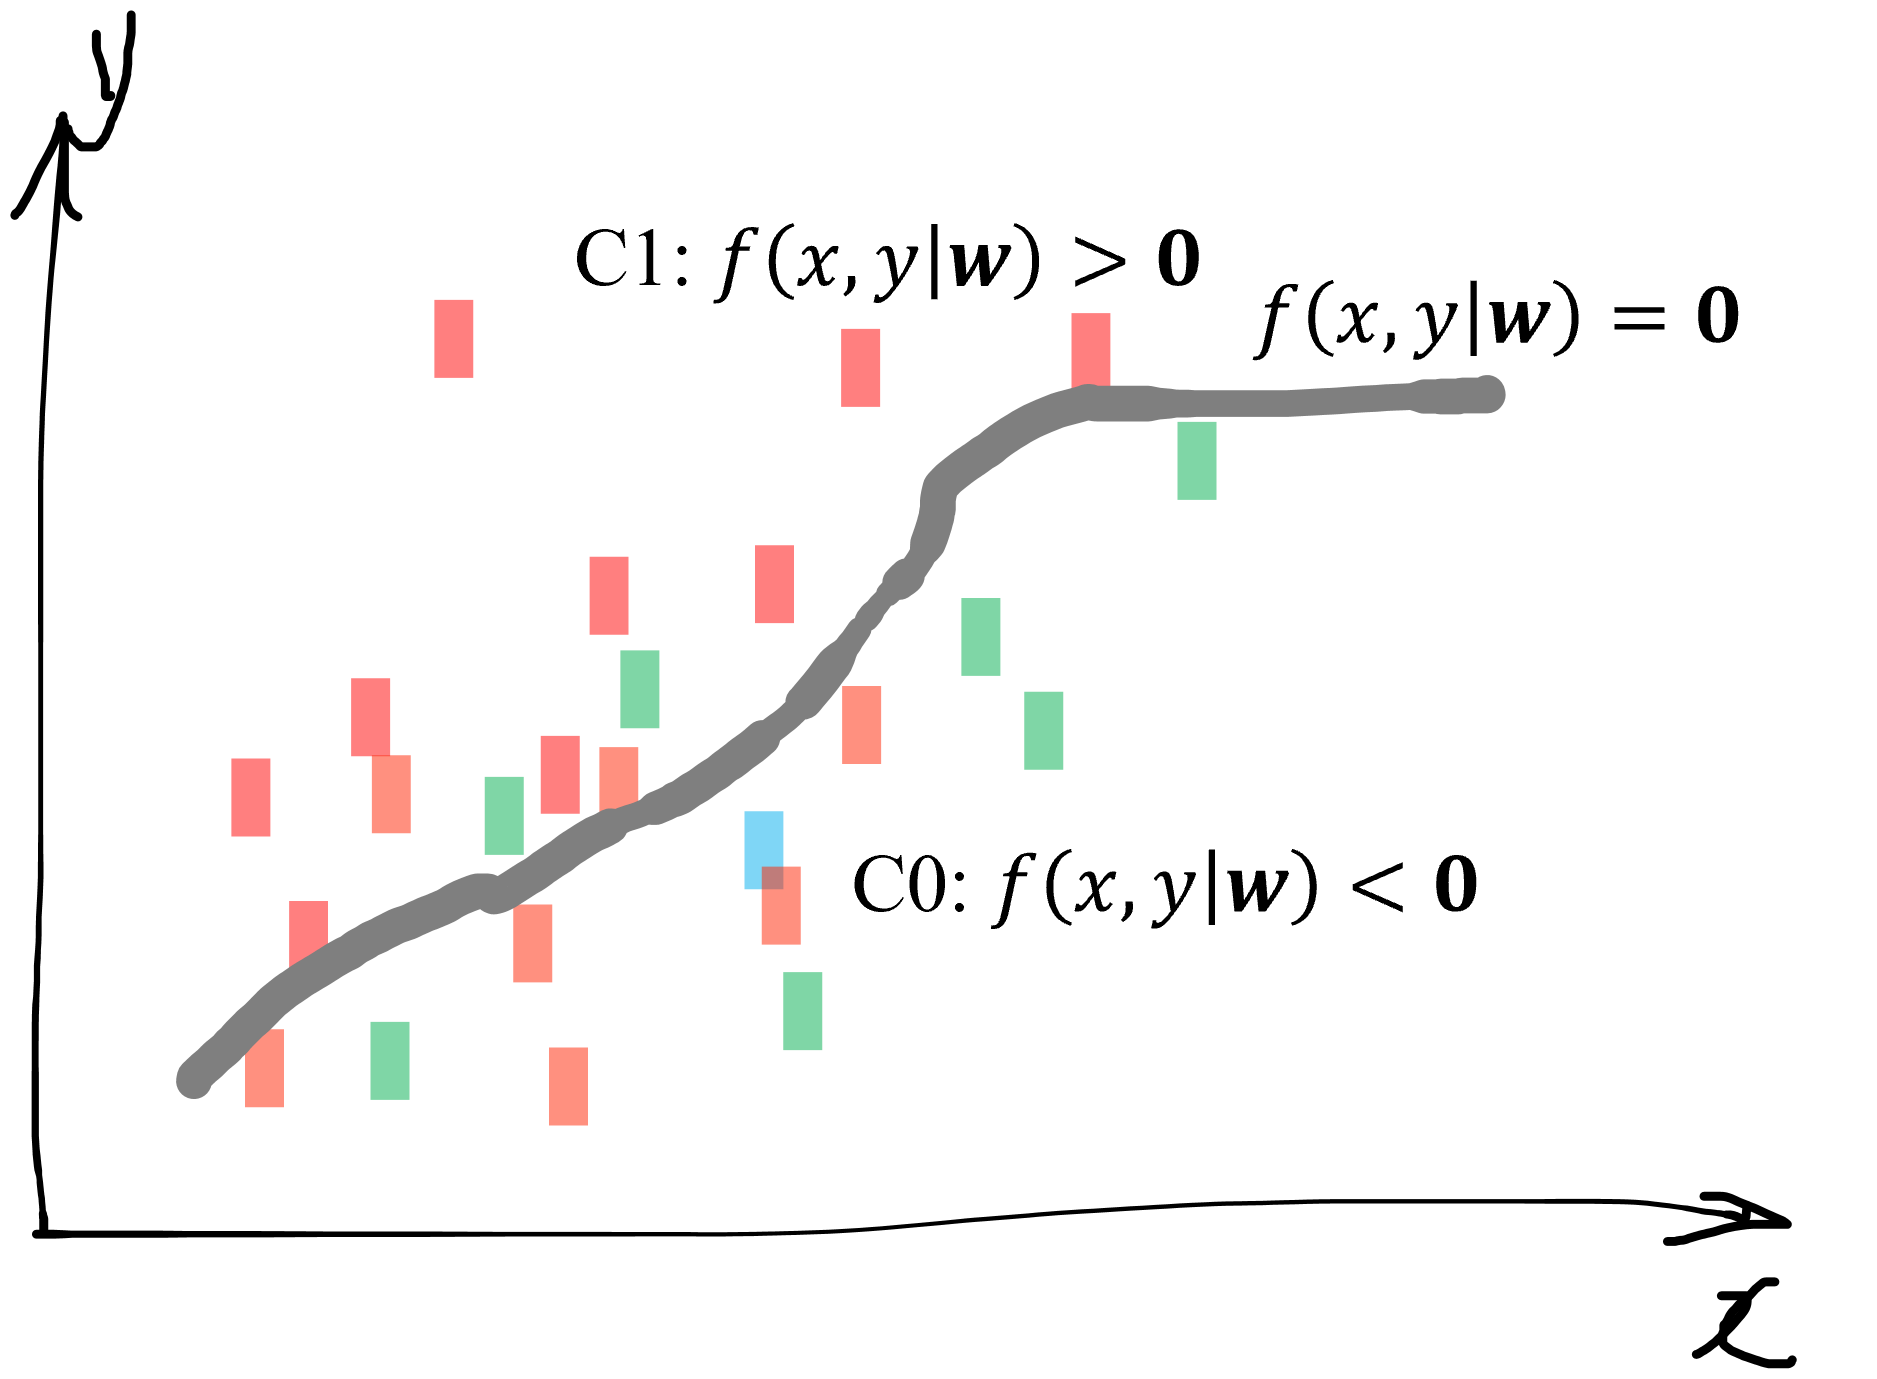
\includegraphics[width=0.55\textwidth]{../figs/nl_boundary.png}
        \caption{Nonlinear decision boundary defined by $f(x, y \mid \bm{w})$.}
    \end{figure}
\end{frame}

\begin{frame}{Complexity in High Dimensions}
    \justifying
    \begin{itemize}
        \item High-dimensional features can yield highly nonlinear decision surfaces.
        \begin{itemize}
            \item It's notorious---often called the \emph{curse of dimensionality}.\footnote{See Wikipedia, \emph{``Curse of dimensionality.''}}
        \end{itemize}
        \item Parameter estimation becomes more challenging with increased complexity.
        \begin{itemize}
            \item Non-parametric methods (e.g., kernel approaches) address this challenge.
        \end{itemize}
    \end{itemize}
\end{frame}

\begin{frame}{Parametric vs. Non-Parametric Models}
    \justifying
    \begin{conceptbox}{Modeling Structures}
        \begin{itemize}
            \item Parametric: fixed dimension of $\bm{w}$, independent of dataset size.
            \item Non-parametric: model complexity grows with the dataset.
        \end{itemize}
    \end{conceptbox}
    \begin{itemize}
        \item Examples: logistic regression vs. SVMs and kernel methods.
    \end{itemize}
\end{frame}

\begin{frame}{Toy Example: Rule-Based vs. Linear Model}
    \justifying
    \begin{examplebox}{Data and Models}
        pH data: $\{7, 7, 6, 2, 2, 14, 8, 5, 7, 1, 14, 1, 1, 1, 9, 4\}$.
        Labels: $\{G, G, G, G, G, B, G, G, B, G, B, G, G, G, G, G\}$.
        Rule-based classifier: threshold at $pH=8.5$.
        Linear discriminative model: $f(x) = -8 + 2x$ (parameters set for illustration).
    \end{examplebox}
\end{frame}

\begin{frame}{Confusion Matrix: Rule-Based Model}
    \justifying
    \[
    \begin{array}{cc|c|c|}
        & \multicolumn{1}{c}{} & \multicolumn{2}{c}{\text{Predicted}} \\ \cline{3-4}
        & \multicolumn{1}{c}{} & \text{Good} & \text{Bad} \\ \cline{3-4}
        \multirow{2}{*}{\rotatebox[origin=c]{90}{\text{Actual}}} & \text{Good} & 12 & 1 \\ \cline{3-4}
        & \text{Bad} & 1 & 2 \\ \cline{3-4}
    \end{array}
    \]
    \begin{itemize}
        \item Overall accuracy: $\text{OA} = \frac{12+2}{16} = 87.5\%$.
    \end{itemize}
\end{frame}

\begin{frame}{Confusion Matrix: Linear Model}
    \justifying
    \[
    \begin{array}{cc|c|c|}
        & \multicolumn{1}{c}{} & \multicolumn{2}{c}{\text{Predicted}} \\ \cline{3-4}
        & \multicolumn{1}{c}{} & \text{Good} & \text{Bad} \\ \cline{3-4}
        \multirow{2}{*}{\rotatebox[origin=c]{90}{\text{Actual}}} & \text{Good} & 6 & 7 \\ \cline{3-4}
        & \text{Bad} & 0 & 3 \\ \cline{3-4}
    \end{array}
    \]
    \begin{itemize}
        \item Overall accuracy: $\text{OA} = \frac{6+3}{16} = 56.3\%$.
        \begin{itemize}
            \item Parameters must be learned from data to be competitive.
        \end{itemize}
    \end{itemize}
\end{frame}

\section{Generative Learning}

\begin{frame}{Generative Learning Formulation}
    \justifying
    \begin{conceptbox}{Definition}
        Generative learning models how data are generated with respect to class labels,
        typically using explicit probabilistic distributions.
    \end{conceptbox}
    \begin{itemize}
        \item Inference is performed via Bayes' rule using learned distributions.
    \end{itemize}
\end{frame}

\begin{frame}{Histogram as a Starting Point}
    \justifying
    \begin{itemize}
        \item Plotting histograms provides an initial impression of the data distribution.
        \item This helps select an appropriate probabilistic model.
        \begin{itemize}
            \item Visual inspection guides the modeling assumptions.
        \end{itemize}
    \end{itemize}
\end{frame}

\begin{frame}{Histogram and Class-Conditional Densities}
    \justifying
    \begin{figure}
        \centering
        \begin{subfigure}[b]{0.46\textwidth}
            \centering
            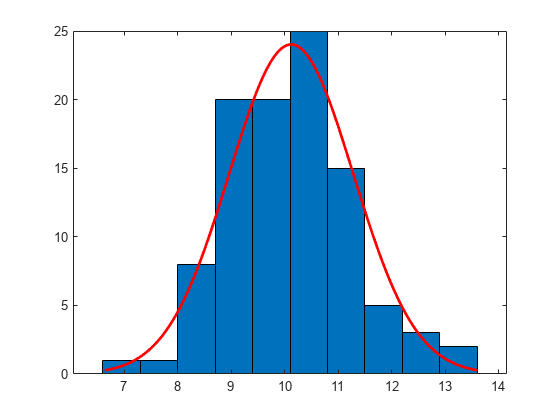
\includegraphics[width=\textwidth]{../figs/histo_distri.png}
            \caption{Histogram of measurements.}
        \end{subfigure}
        \hfill
        \begin{subfigure}[b]{0.46\textwidth}
            \centering
            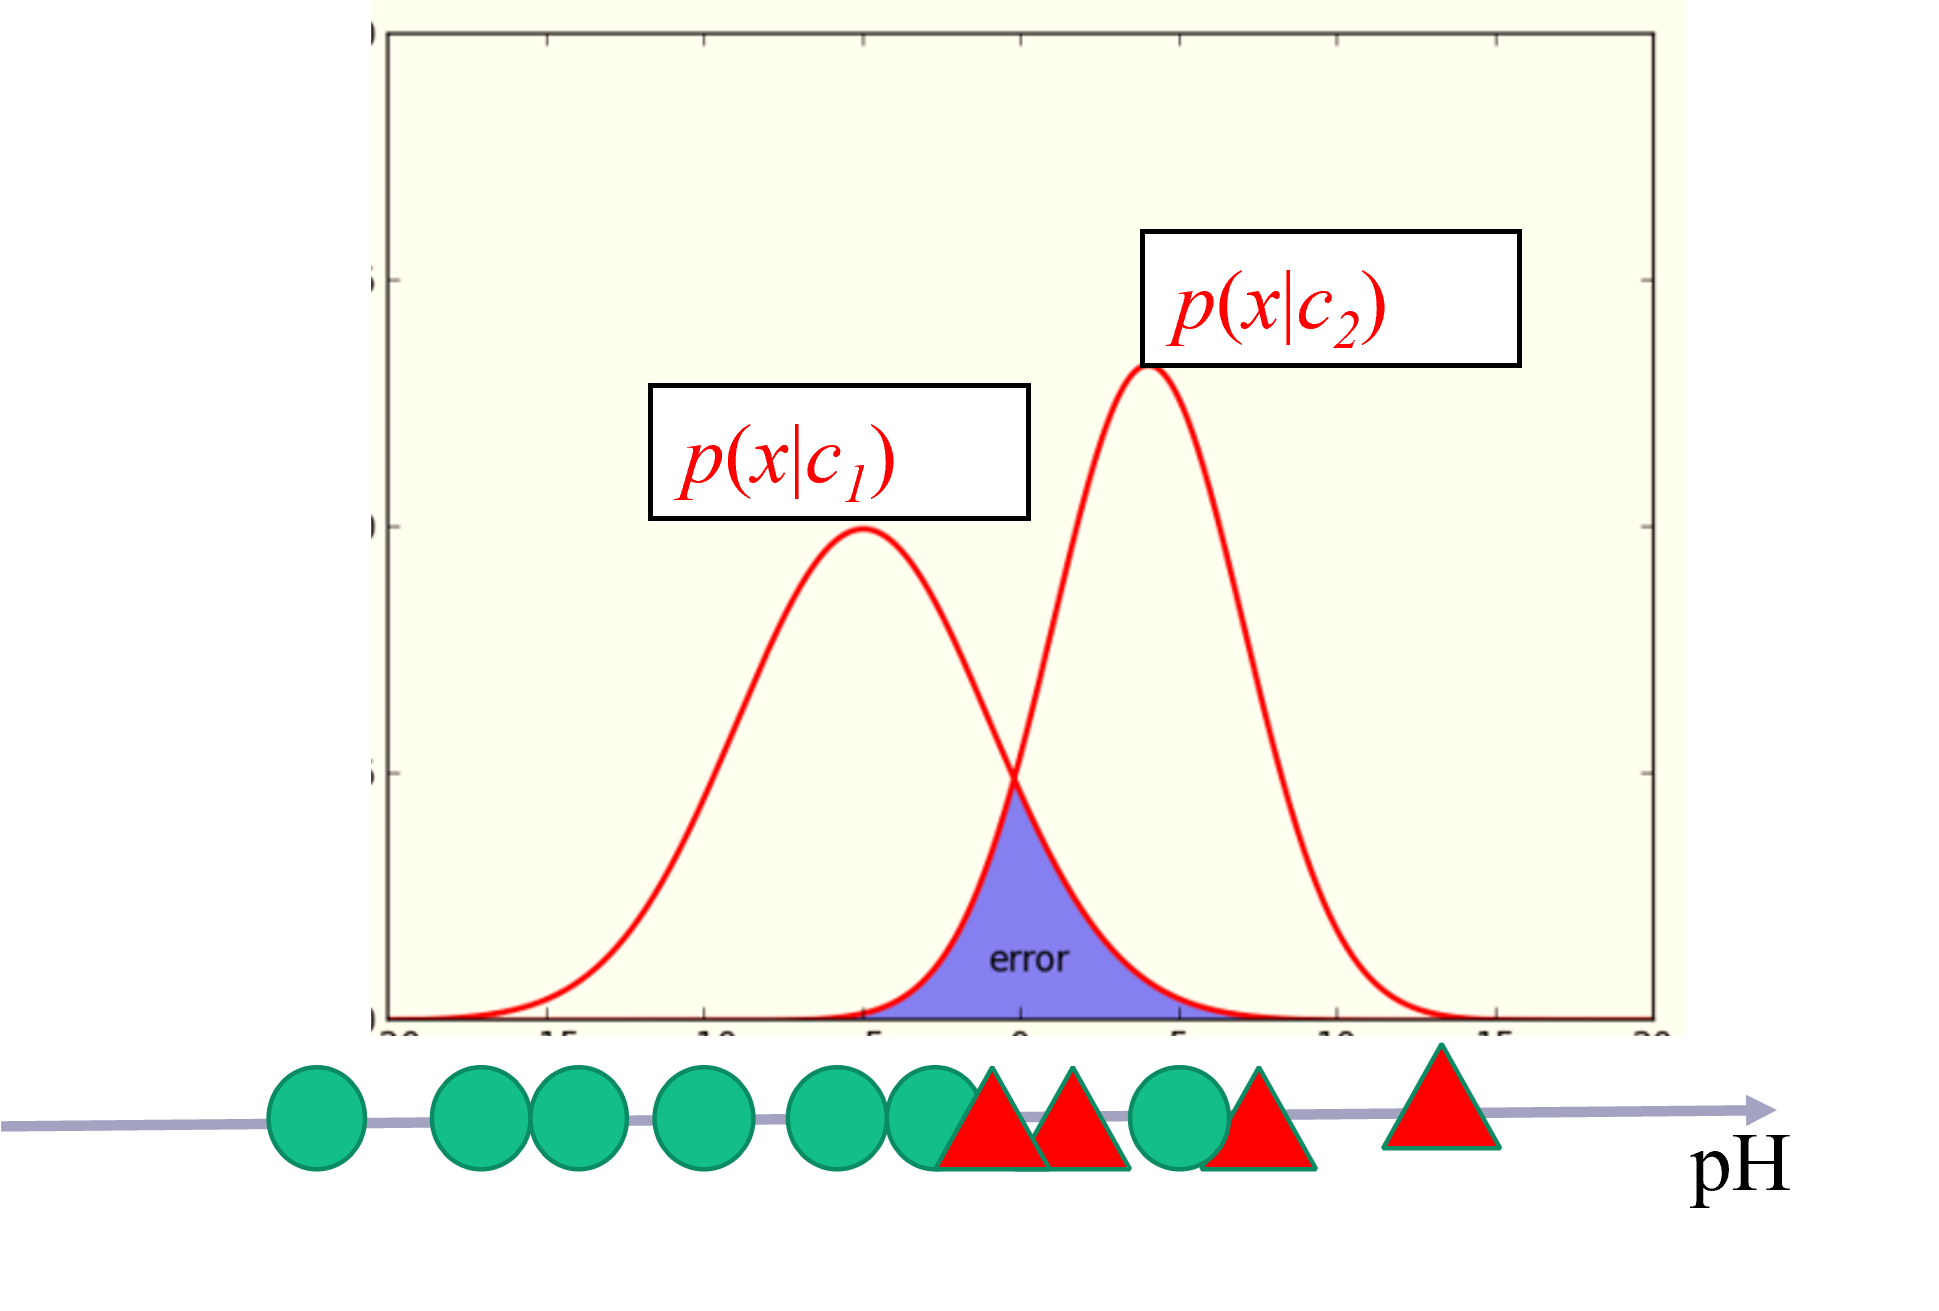
\includegraphics[width=\textwidth]{../figs/bayes.png}
            \caption{Class-conditional densities.}
        \end{subfigure}
        \caption{Histogram and illustrative class-conditional distributions.}
    \end{figure}
\end{frame}

\begin{frame}{Probability Models in Generative Learning}
    \justifying
    \begin{itemize}
        \item Use parametric PDFs such as Gaussian or exponential family distributions.
        \item For each class $c$, model $p(x \mid c)$.
        \item Any PDF must satisfy $\int_{-\infty}^{\infty} p(x \mid c) \, dx = 1$.
    \end{itemize}
\end{frame}

\begin{frame}{Class Priors as a PMF}
    \justifying
    \begin{itemize}
        \item Class labels are categorical, so use a PMF $P(c)$.
        \item The PMF must satisfy $\sum_c P(c) = 1$.
        \begin{itemize}
            \item For binary labels: $P(c=1) + P(c=0) = 1$.
        \end{itemize}
    \end{itemize}
\end{frame}

\begin{frame}{Bayes' Theorem for Classification}
    \justifying
    \begin{conceptbox}{Bayes' Rule}
        \begin{equation}
        P(c \mid x) = \frac{p(x \mid c)P(c)}{p(x)}.
        \end{equation}
    \end{conceptbox}
    \begin{itemize}
        \item $p(x \mid c)$: likelihood, $P(c)$: prior, $P(c \mid x)$: posterior.
    \end{itemize}
    \vspace{0.5em}
    {\footnotesize Source: \url{https://ocw.mit.edu/courses/18-05-introduction-to-probability-and-statistics-spring-2022/mit18_05_s22_class11-prep.pdf}}
\end{frame}

\begin{frame}{Decision Rule from Bayes' Theorem}
    \justifying
    \begin{itemize}
        \item Since $p(x)$ does not depend on $c$, it acts as a normalization constant.
        \item Therefore $P(c \mid x) \propto p(x \mid c) P(c)$.
        \item Prediction is made by
        \[c^* = \mathrm{argmax}_c\, p(x \mid c)P(c).\]
    \end{itemize}
\end{frame}

\begin{frame}{Toy Example: Coin Tossing (Setup)}
    \justifying
    \begin{itemize}
        \item Two classes: $c \in \{H, T\}$.
        \item Discrete measurement: $x \in \{-1, 1\}$, where $x=1$ is Heads.
        \item 1000 labeled observations yield priors $P(H)=0.8$, $P(T)=0.2$.
        \begin{itemize}
            \item This avoids continuous density modeling while illustrating Bayes' rule.
        \end{itemize}
    \end{itemize}
\end{frame}

\begin{frame}{Toy Example: Conditional Probabilities}
    \justifying
    \begin{itemize}
        \item $P(x=-1 \mid H) = 0.7$, $P(x=1 \mid H) = 0.3$.
        \item $P(x=-1 \mid T) = 0.2$, $P(x=1 \mid T) = 0.8$.
        \begin{itemize}
            \item These are estimated from labeled observations.
        \end{itemize}
    \end{itemize}
\end{frame}

\begin{frame}{Toy Example: Inference}
    \justifying
    \begin{itemize}
        \item For $x=1$, compute $P(x=1)=0.3\times0.8+0.8\times0.2=0.4$.
        \item Posterior probabilities: $P(H \mid x=1)=0.6$, $P(T \mid x=1)=0.4$.
        \item Classify as $H$ because $P(H \mid x=1)$ is larger.
    \end{itemize}
\end{frame}

\begin{frame}{Generative Learning vs. Generative AI}
    \justifying
    \begin{itemize}
        \item Generative learning: explicit probabilistic models of $p(x \mid c)$ and $P(c)$.
        \item Generative AI: foundation-scale neural models that synthesize data.
        \begin{itemize}
            \item The term ``generative'' spans distinct eras and modeling assumptions.
        \end{itemize}
    \end{itemize}
\end{frame}

\begin{frame}{Modern Generative AI Training Stages}
    \justifying
    \begin{conceptbox}{Typical Training Pipeline}
        \begin{itemize}
            \item Self-supervised pretraining on massive datasets.
            \item Supervised fine-tuning for task adaptation.
            \item Preference optimization (e.g., RLHF) for alignment.
        \end{itemize}
    \end{conceptbox}
    \vspace{0.5em}
    {\footnotesize Sources: \url{https://arxiv.org/abs/2005.14165};
    \url{https://cdn.openai.com/papers/Training_language_models_to_follow_instructions_with_human_feedback.pdf}}
\end{frame}

\section{Conclusion Remarks}

\begin{frame}{Summary: ML Paradigms}
    \justifying
    \begin{itemize}
        \item ML is the dominant data-enabled paradigm of modern AI.
        \item Three core paradigms: supervised, unsupervised, and reinforcement learning.
        \item Learning is inductive during training and deductive during inference.
    \end{itemize}
\end{frame}

\begin{frame}{Summary: Learning Formalisms}
    \justifying
    \begin{itemize}
        \item Discriminative learning: decision boundaries or $P(c \mid x)$ directly.
        \item Generative learning: model data generation with $p(x \mid c)$ and $P(c)$.
        \item Bayes' rule enables probabilistic inference from learned models.
    \end{itemize}
\end{frame}

\begin{frame}{What Comes Next}
    \justifying
    \begin{itemize}
        \item Develop concrete discriminative models: logistic regression, neural networks, SVMs.
        \item Study optimization and generalization theory in supervised learning.
        \item Connect classical foundations to modern deep and generative models.
    \end{itemize}
\end{frame}

\begin{frame}{Key References}
    \justifying
    \begin{itemize}
        \item Cornell CS4780 Supervised Learning: \url{https://www.cs.cornell.edu/courses/cs4780/2018fa/lectures/lecturenote01_MLsetup.html}
        \item MIT Intro ML Notes (Unsupervised): \url{https://introml.mit.edu/_static/spring24/LectureNotes/chapter_Unsupervised_Learning.pdf}
        \item MIT Intro ML Notes (RL): \url{https://introml.mit.edu/notes/reinforcement_learning.html}
        \item MIT OCW 18.05 Bayes' Theorem: \url{https://ocw.mit.edu/courses/18-05-introduction-to-probability-and-statistics-spring-2022/mit18_05_s22_class11-prep.pdf}
        \item EPA Secondary Drinking Water Standards: \url{https://www.epa.gov/sdwa/secondary-drinking-water-standards-guidance-nuisance-chemicals}
        \item GPT-3 and InstructGPT Papers: \url{https://arxiv.org/abs/2005.14165},
        \url{https://cdn.openai.com/papers/Training_language_models_to_follow_instructions_with_human_feedback.pdf}
    \end{itemize}
\end{frame}

\end{document}
